% !TeX spellcheck = en_US
\documentclass[a4paper,12pt]{article}
\usepackage{listings}
%\usepackage[T1]{fontenc}
\usepackage{fontspec}
\usepackage[greek, english]{babel}
\usepackage[super]{nth}
\usepackage{fancyhdr}
\usepackage[left=1.50cm, right=1.50cm, top=2cm, bottom=1.cm, includeheadfoot]{geometry}
\usepackage{amsmath}
\usepackage{graphicx}
\usepackage{subcaption}
\usepackage{float}
%\usepackage[colorinlistoftodos]{todonotes}
\usepackage{xcolor}
\usepackage{ulem}
\usepackage{amsmath}
\usepackage{caption}
\usepackage{subcaption}
\usepackage{tabularray}
\usepackage[framed]{matlab-prettifier}
\usepackage{svg}
\usepackage{nth}
\usepackage{wrapfig}

\usepackage[pdfauthor={Alexandra Gianni, Nikos Stylianou},
pdftitle={First Problem Set},
pdfcreator={TeX},
pdfsubject={ECE447 - Neuro-Fuzzy Computing}]{hyperref}


\hypersetup{
	colorlinks,
	citecolor=blue,
	filecolor=black,
	linkcolor=black,
	urlcolor=blue
}

\lstset{
	style              = Matlab-editor,
	basicstyle         = \footnotesize,
	escapechar         = ",
	mlshowsectionrules = true,
}

\setmainfont{Times New Roman}

\pagestyle{fancy}
\fancyhf{}
\fancyhead[l]{\footnotesize \nth{1} Problem Set}
\fancyhead[r]{\footnotesize Neuro-Fuzzy Computing}
%\fancyfoot[r]{\footnotesize \thepage}
\renewcommand{\footrulewidth}{0.4pt} % Line at the footer visible

\fancyfoot[c]{\thepage}

\fancypagestyle{first}{
	\fancyhf{}
	\renewcommand{\headrulewidth}{0pt}
	\fancyfoot[c]{{\large \today}}
	\renewcommand{\footrulewidth}{0.0pt} % Line at the footer visible
} 

\newcommand{\MathSpace}{\ }
\setlength{\parindent}{0pt} % Paragraph identation is set to 0

\newcommand\ddfrac[2]{\frac{\displaystyle #1}{\displaystyle #2}} % Better fractions for inline

\renewcommand{\thesubsection}{(\alph{subsection})} % Change subsection style
\renewcommand{\thesection}{\hspace{-18pt}} % Make section style look nicer

\begin{document}
	
	\begin{titlepage}
		\thispagestyle{first}
		
		\newcommand{\HRule}{\rule{\linewidth}{0.5mm}} % Defines a new command for the horizontal lines, change thickness here
		
		\center % Center everything on the page
		
		%----------------------------------------------------------------------------------------
		%	HEADING SECTIONS
		%----------------------------------------------------------------------------------------
		
		\textsc{\LARGE University of Thessaly}\\[1.6cm] % Name of your university/college
		
\includegraphics[scale=.5]{Images/uth-logo.png}\\[1cm] % Include a department/university logo - this will require the graphicx package
		\textsc{\Large Neuro-Fuzzy Computing}\\[0.6cm] % Major heading such as course name
		\textsc{\large ECE447}\\[0.5cm] % Minor heading such as course title
		
		%----------------------------------------------------------------------------------------
		%	TITLE SECTION
		%----------------------------------------------------------------------------------------
		
		\HRule \\[0.5cm]
		{ \huge \nth{1} Problem Set}\\[0.4cm] % Title of your document
		\HRule \\[1.8cm]
		
		%----------------------------------------------------------------------------------------
		%	AUTHOR SECTION
		%----------------------------------------------------------------------------------------
		
		
		\vspace*{1cm}
		\begin{minipage}{\textwidth}
			\centering
			\begin{tblr}{cc}
				 \emph{{\LARGE Alexandra Gianni}} & \emph{{\LARGE Nikos Stylianou}} \\ [3mm]
				 \emph{{\LARGE ID: 3382}} & \emph{{\LARGE ID: 2917}} \\
			\end{tblr}
		\end{minipage}\\[2.5cm]
		
		% If you don't want a supervisor, uncomment the two lines below and remove the section above
		%\Large \emph{Author:}\\
		%John \textsc{Smith}\\[3cm] % Your name
		
		%----------------------------------------------------------------------------------------
		%	DATE SECTION
		%----------------------------------------------------------------------------------------
		
		
		%\vfill % Fill the rest of the page with whitespace
		
	\end{titlepage}
	
	% !TeX spellcheck = en_US
\section{Problem 1}

Contour lines of $f(x,y)$ are plotted with the following MATLAB code and are presented in figure~\ref{fig:prob_1_contour_lines}.

\begin{lstlisting}[]
function [Z] = plot_contour(start_num, end_num)
	
	x = linspace(start_num, end_num, 100);
	y = x;
	[X, Y] = meshgrid(x, y);
	Z = X.^2 + 4*X.*Y + Y.^2;
	contour(X, Y, Z, 40);
	xlabel('X');
	ylabel('Y');
end
\end{lstlisting}
\begin{figure}[h]
	\centering
	\begin{subfigure}{0.4\textwidth}
		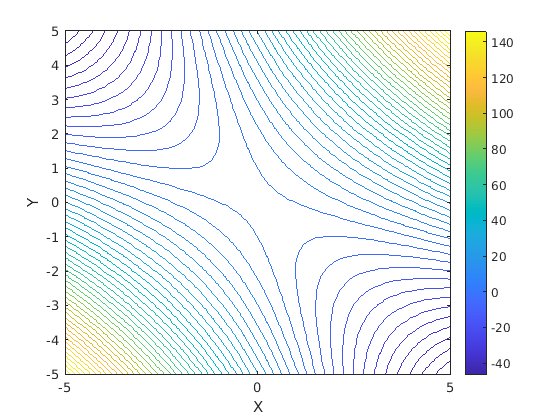
\includegraphics[width=\textwidth]{../Problem 1/contour_lines_2d.png}
		\caption{2D Plot}
		\label{fig:prob_1_contour_lines_2d}
	\end{subfigure}
	\begin{subfigure}{0.4\textwidth}
		\includesvg[width=\textwidth]{../Problem 1/contour_lines_3d.svg}
		\caption{3D Plot}
		\label{fig:prob_1_contour_lines_3d}
	\end{subfigure}
	\caption{Contour lines of $f(x,y)$ }
	\label{fig:prob_1_contour_lines}
\end{figure}

A general formula of a quadratic equation is $f(x,y) = ax^2 + 2bxy + cy^2$. Writing our formula in the previous form, we find that $a=1, \MathSpace b=2, \MathSpace c=1$.
Calculation of discriminant can help us calculate the location of function's local minimum/maximum.

\begin{equation}
\begin{gathered}
D =
\left[
\begin{array}{cc}
	f_{xx} & f_{xy} \\
	f_{yx} & f_{yy} \\
\end{array}
\right]
= f_{xx} f_{yy} - f^2_{xy} = 2 \times 2 - 4^2 = -12 < 0, \quad \text{όπου} \\
f_{xx} = \frac{\partial^2 f}{\partial x^2} = 2, \quad
f_{yy} = \frac{\partial^2 f}{\partial y^2} = 2, \quad
f_{xy} = \frac{\partial}{\partial y} \left( \frac{\partial f}{\partial x} \right) = 4
D = 2 \times 2 - 4^2 = -12 < 0.
\end{gathered}
\end{equation}

So, we only have to find the point where $\frac{\partial f}{\partial x}$ and $\frac{\partial f}{\partial y}$ are equal to $0$. Thus, this point will be a saddle point where gradients in each orthogonal direction are $0$, but this point is not either a local minimum or maximum.
Specifically:
\begin{equation}
\left\{
\begin{array}{c}
	\frac{\partial f}{\partial x} = 2x + 4y = 0 \\ 
	\frac{\partial f}{\partial y} = 4x + 2y = 0 \\
\end{array}
\right.
\Rightarrow
\left\{
\begin{array}{c}
	x = 0\\y=0\\
\end{array}
\right.
\end{equation}
Thus, the point $(x,y) = (0,0)$ is the saddle point mentioned before for the function given and this can be justified using the plotted contour lines.
	\input{Sources/problem2.tex}
	% !TeX spellcheck = en_US
\section{Problem 3}

Henon map is a dynamic system described by the recursive equation 
\[
x_{k+1} = 1 - ax^2_k + bx_{k-1}
\]

A lot of dynamic systems transition into chaos as gain or control is increased to a certain point and this system falls into this category.
In this problem, we will plot the trajectories of sequences $x_0 ... x_i$ and describe it.

The first parameters are (a,b) = (0.3, 0.4) and the trajectories of the sequences are presented in figure~\ref{fig:prob3_x_init}.

\begin{figure}[htpb]
	\centering
	\begin{subfigure}{.47\textwidth}
		\centering
		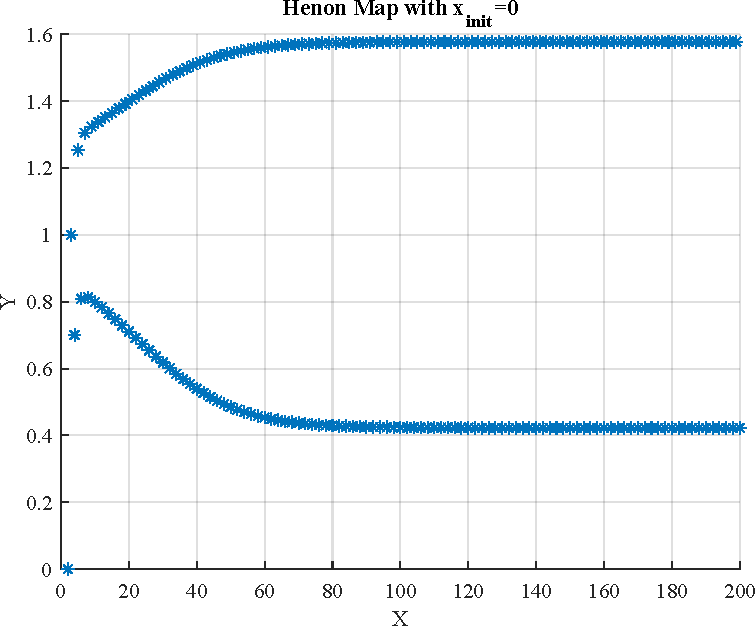
\includegraphics[width=\textwidth]{../Problem 3/prob3_x_init_0.pdf}
		\caption{}
	\end{subfigure}
	\hspace{1mm}
	\begin{subfigure}{.47\textwidth}
		\centering
		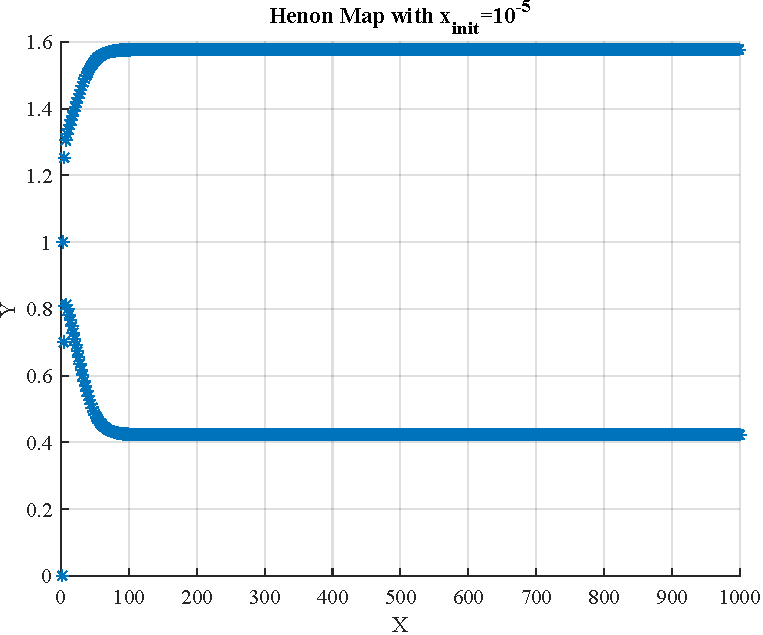
\includegraphics[width=\textwidth]{../Problem 3/prob3_x_init_1e-5.pdf}
		\caption{}
	\end{subfigure}
	\caption{Trajectories of Henon map's sequence with (a,b) = (0.3, 0.4)}
	\label{fig:prob3_x_init}
\end{figure}
From the produced plots, this system with parameters (0.3, 0.4) is periodic after converging.

\subsection{Multiple a values}
Figure~\ref{fig:prob3_multiple_a} shows output of the sequence for different values of $a$ and $b=0$. When $a \le 0.6$, the output swings for a bit and then stabilizes to a fixed number, with that number decreasing while $a$ approaches $0.6$.


\begin{figure}[htpb]
	\centering
	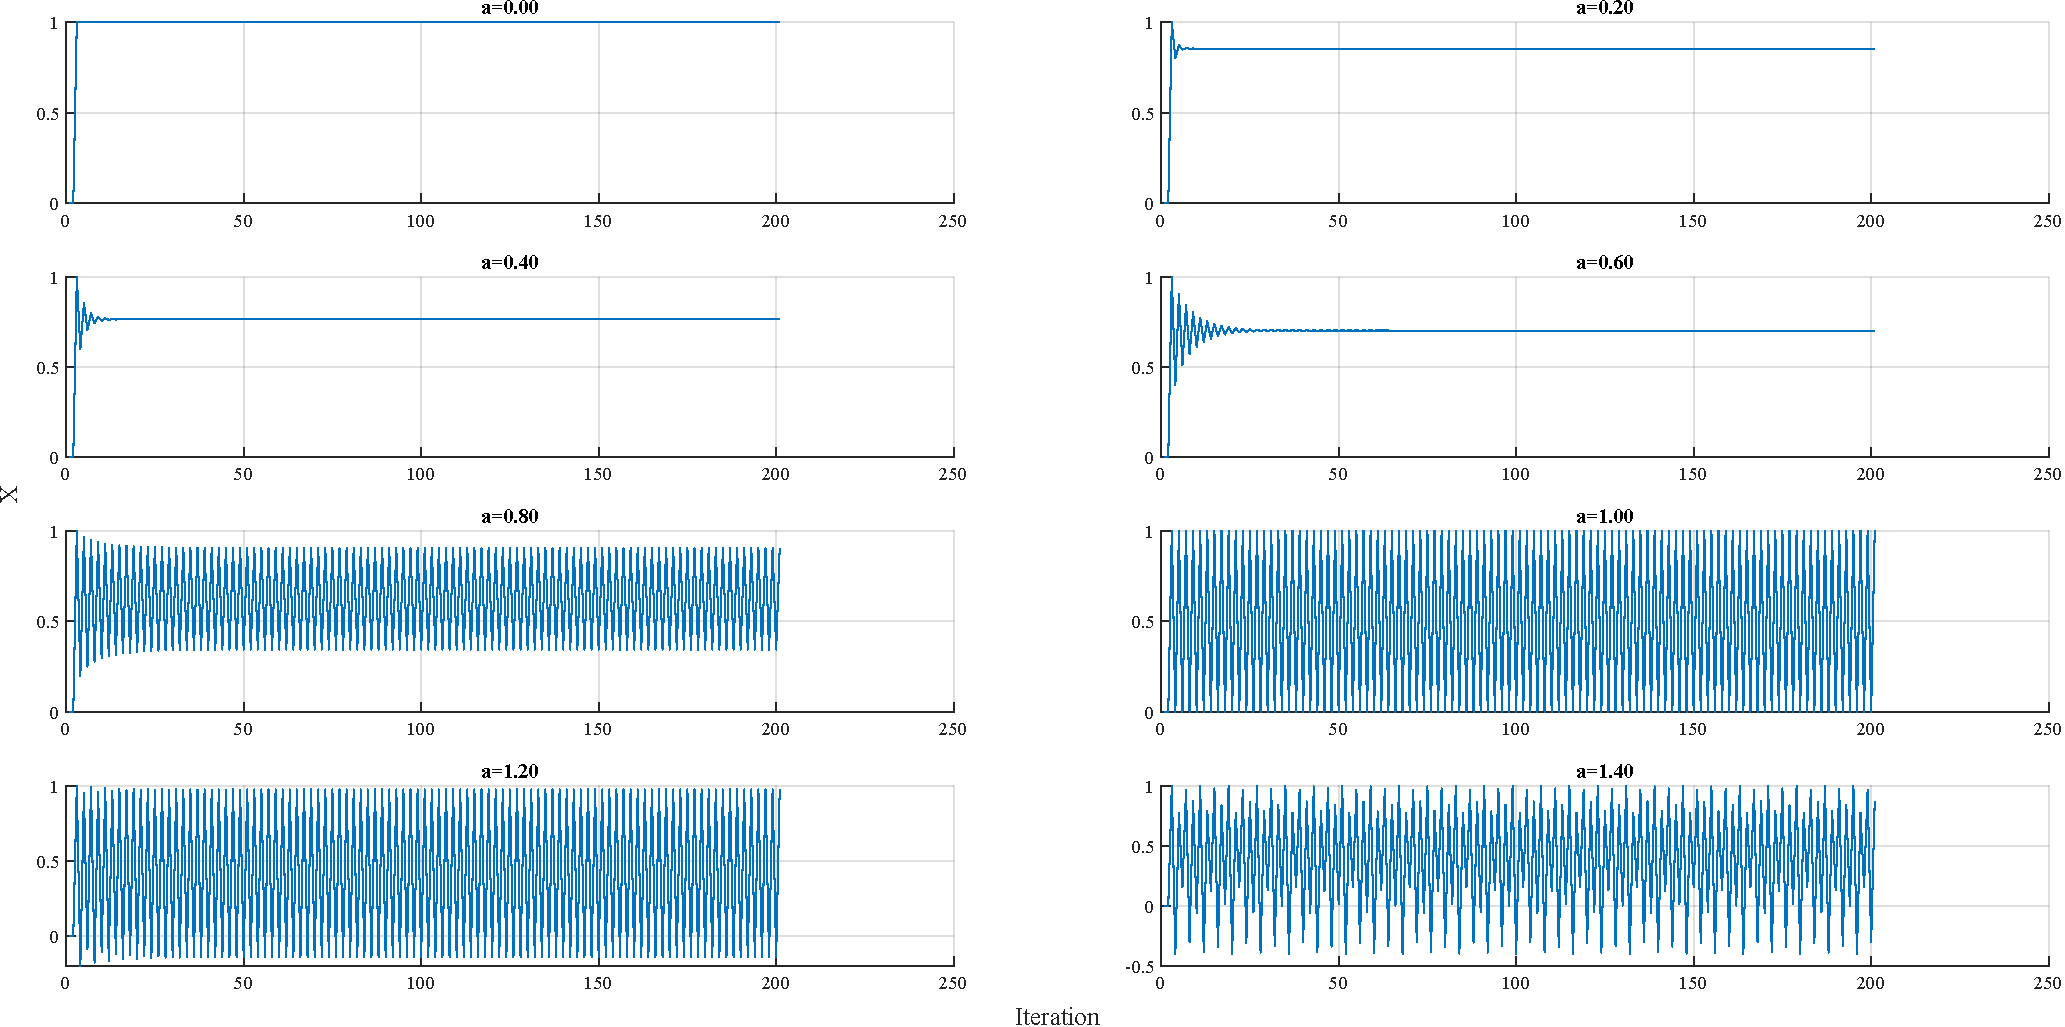
\includegraphics[width=\textwidth]{../Problem 3/prob3_(a)_multiple_a_b_0.pdf}
	\caption{Sequence output for different $a$ and $b=0$}
	\label{fig:prob3_multiple_a}
\end{figure}

When $a \ge 0.8$, output starts to oscillate. As $a$ approaches $1$, the oscillation's amplitude is getting bigger until it reaches value $1$.
After $a$ surpasses $1$, the oscillation starts to break down, as shown in the last two sub-figures. The greater $a$, the greater the disturbance on the oscillation thus chaos is created.

\subsection{Multiple initial x values}

Figure~\ref{fig:prob3_multiple_x_multiple_b} shows the trajectory of sequences with different $x_{init}$ and $b$, with $a = c, \ \text{where} \ c = 0.3$ from previous question.
Inspecting this figure, we can understand some things about those parameters and what they affect on the system, as even with $b=0$, the system performs a damped oscillation for the first 50 (at most) $x_i$.
For a given $x_{init}$ (ie. $0$), increasing $b$ increases the amplitude of oscillation as well as the overshoot percentage (if we see it as an system response).

\textit{\footnotesize PS: Overshoot \% is the percentage of system's maximum value that surpasses its steady-state value over the latter.}


\begin{figure}[htpb]
	\centering
	\begin{subfigure}{0.47\textwidth}
		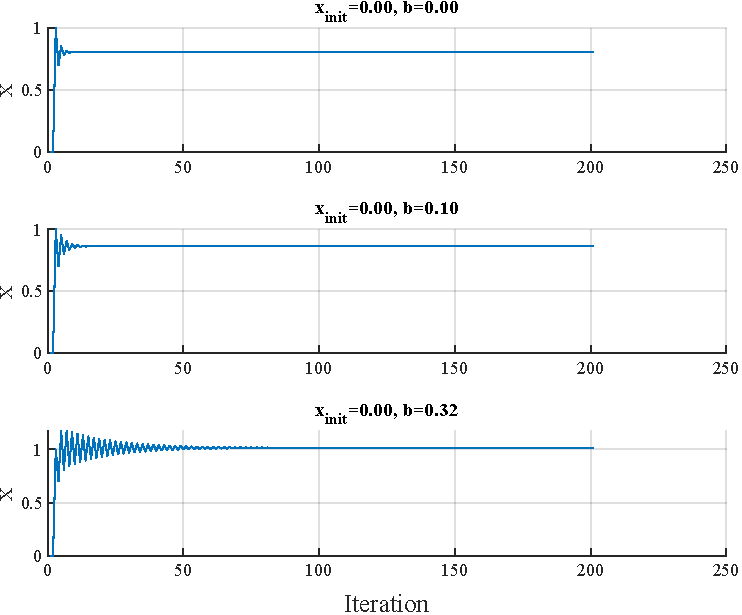
\includegraphics[width=\textwidth]{../Problem 3/prob3_(b)_x_init_0.00.pdf}
		\caption{}
	\end{subfigure}
	\begin{subfigure}{0.47\textwidth}
		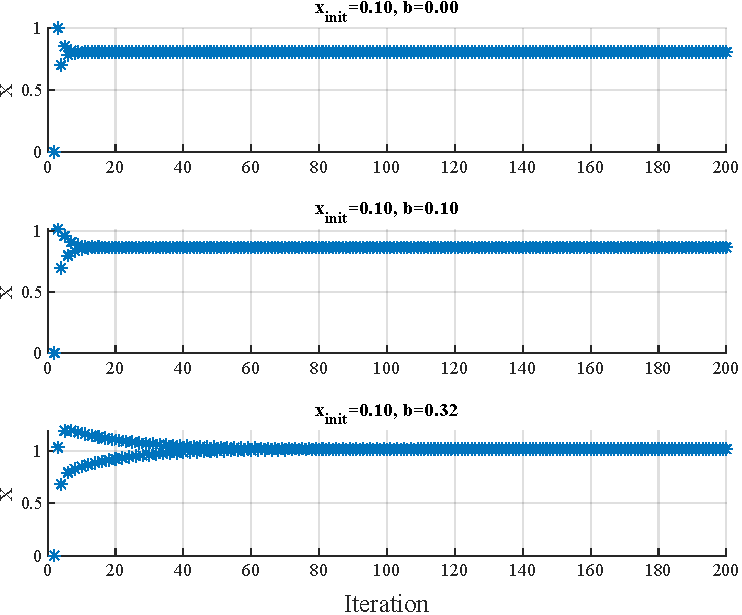
\includegraphics[width=\textwidth]{../Problem 3/prob3_(b)_x_init_0.10.pdf}
		\caption{}
	\end{subfigure}\\[4mm]
	\begin{subfigure}{0.47\textwidth}
		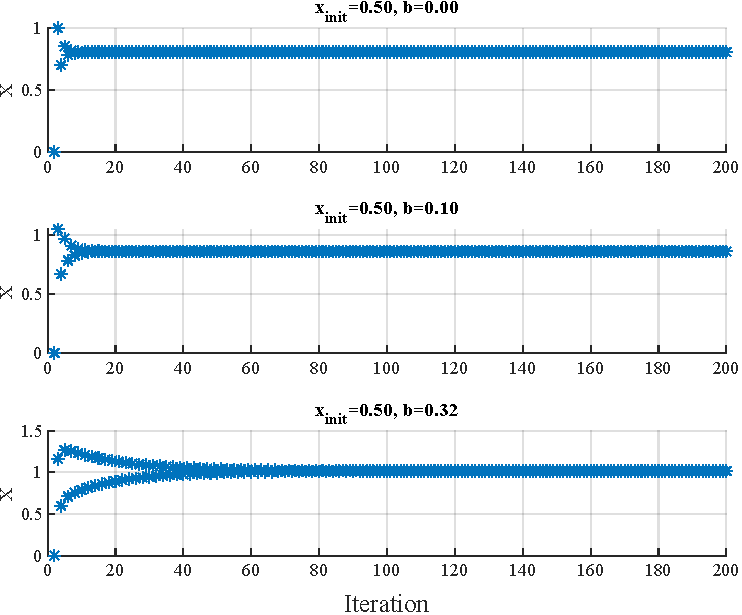
\includegraphics[width=\textwidth]{../Problem 3/prob3_(b)_x_init_0.50.pdf}
		\caption{}
	\end{subfigure}
	\begin{subfigure}{0.47\textwidth}
		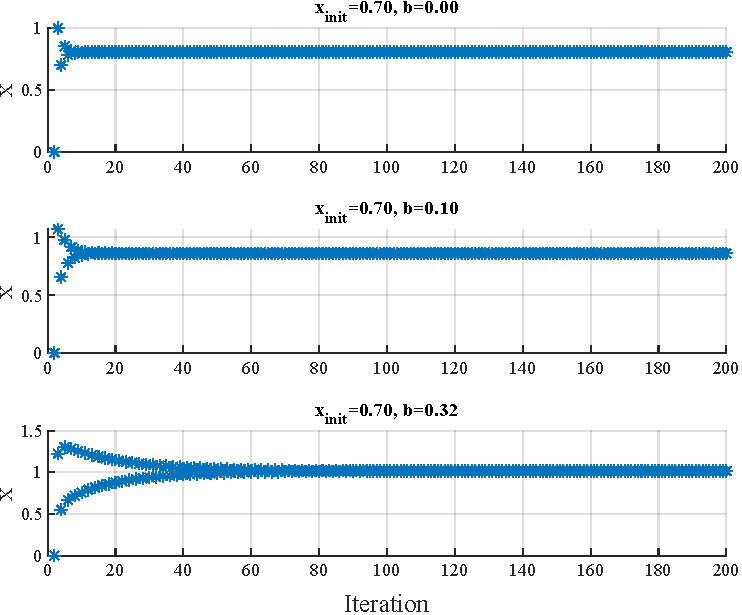
\includegraphics[width=\textwidth]{../Problem 3/prob3_(b)_x_init_0.70.pdf}
		\caption{}
	\end{subfigure}\\[4mm]
	\begin{subfigure}{0.47\textwidth}
		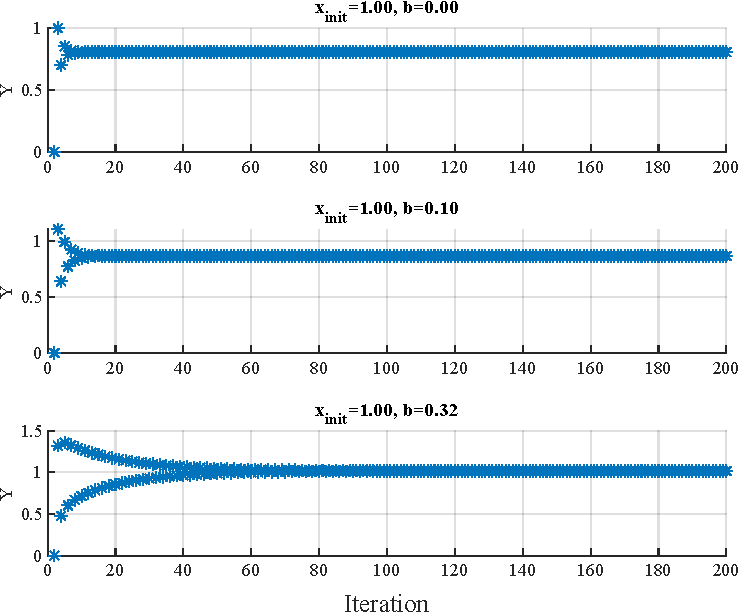
\includegraphics[width=\textwidth]{../Problem 3/prob3_(b)_x_init_1.00.pdf}
		\caption{}
	\end{subfigure}
	\caption{}
	\label{fig:prob3_multiple_x_multiple_b}
\end{figure}

\subsection{(a,b) = (0.3675, 0.3)}

By setting these values to the system, we observe that the sequence starts to oscillate with a very high frequency. As the sequence progresses, the observed oscillation's amplitude dampens and settles around a fixed number, whilst still oscillating.

\begin{figure}[htpb]
	\centering
	\begin{subfigure}{0.4\textwidth}
		\centering
		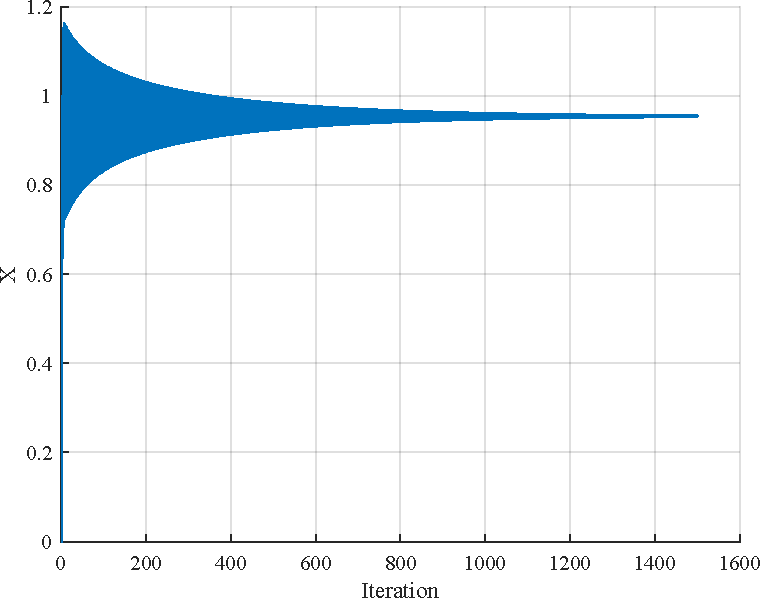
\includegraphics[width=\textwidth]{../Problem 3/prob3_(c)_a_0.365_b_0.3.pdf}
		\caption{Normal trajectory}
	\end{subfigure}
	\begin{subfigure}{0.4\textwidth}
		\centering
		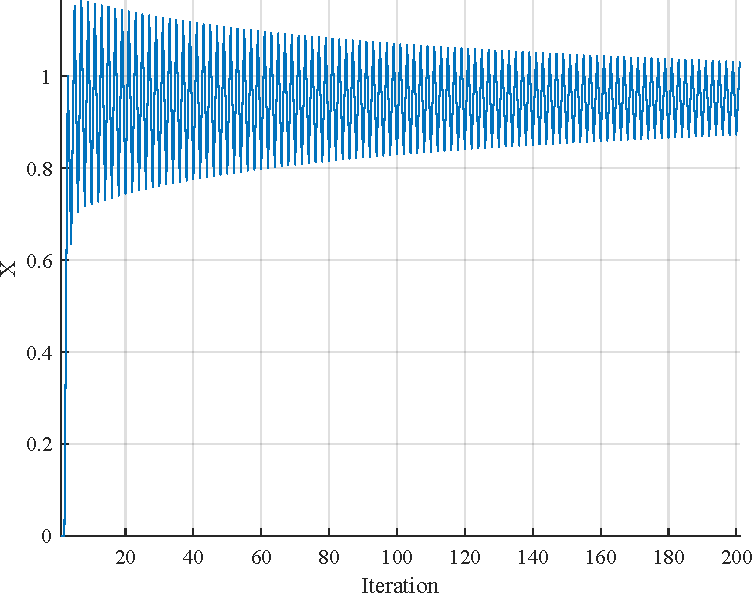
\includegraphics[width=\textwidth]{../Problem 3/prob3_(c)_a_0.365_b_0.3_zoomed.pdf}
		\caption{Zoomed in}
	\end{subfigure}
	\caption{Sequence's trajectory with (0.3675, 0.3)}
\end{figure}

\subsection{Multiple a values}

By changing $a$ parameter, we can spot and characterize system's output. Observing figure~\ref{fig:prob3_d_multiple_a}, we understand that increasing the parameter's value increases oscillation duration. At first, (when $a$ is smaller to $b$), the system oscillates for a bit and then dampens around a fixed number. But as $a$ approaches $b$, oscillation duration gets bigger until the moment where $a=b$.
From this value and over, oscillation lasts for all $x_i$. As $a$ increases beyond $b$, the oscillations begin to deteriorate, and beyond a certain point of a, chaos ensues.
\begin{figure}[htbp]
	\centering
	\begin{subfigure}{0.3\textwidth}
		\centering
		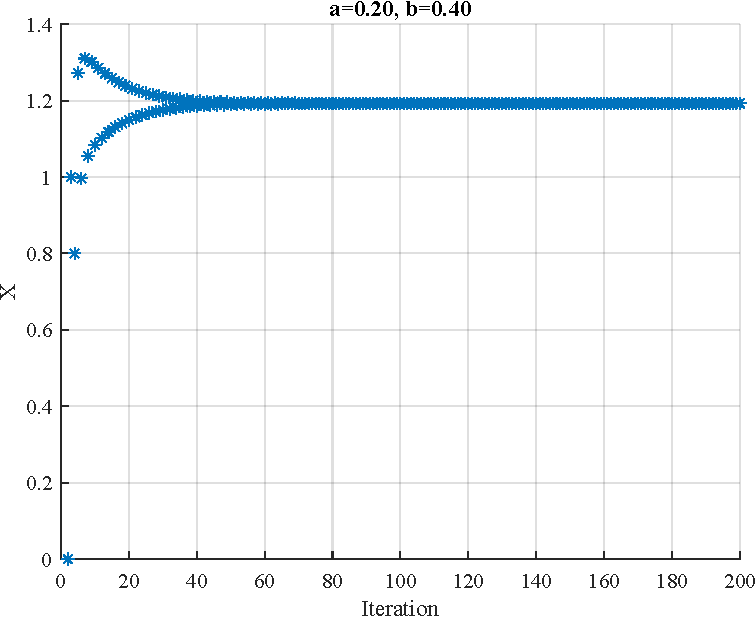
\includegraphics[width=\textwidth]{../Problem 3/prob3_(d)_a_0.20_b_0.40.pdf}
		\caption{}
	\end{subfigure}
	\begin{subfigure}{0.3\textwidth}
		\centering
		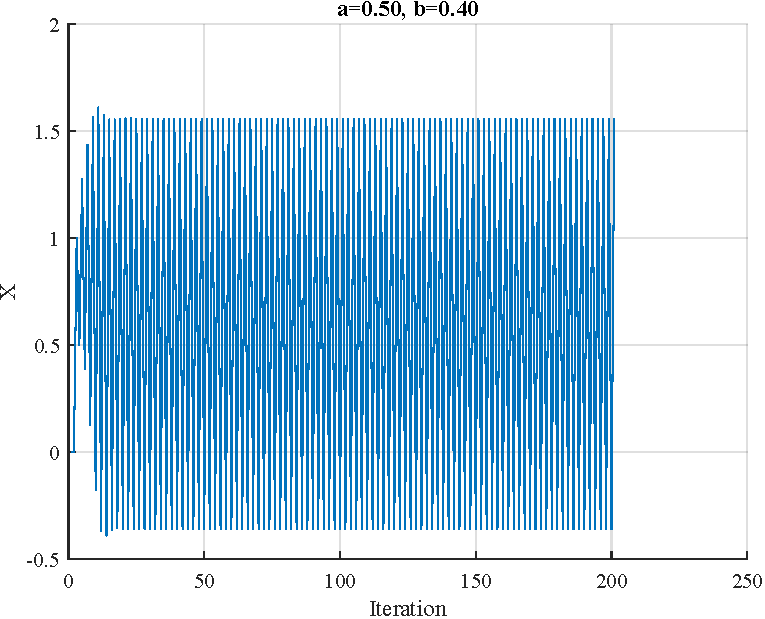
\includegraphics[width=\textwidth]{../Problem 3/prob3_(d)_a_0.50_b_0.40.pdf}
		\caption{}
	\end{subfigure}
	\begin{subfigure}{0.3\textwidth}
		\centering
		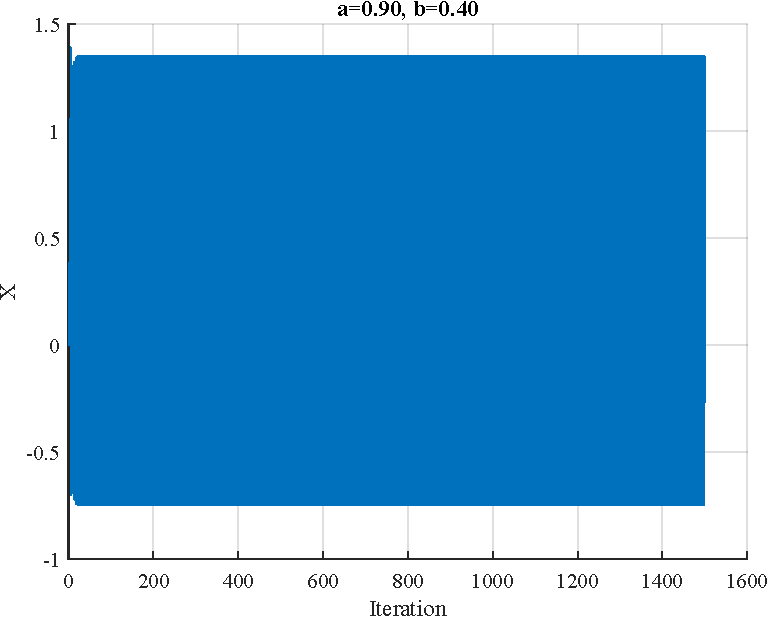
\includegraphics[width=\textwidth]{../Problem 3/prob3_(d)_a_0.90_b_0.40.pdf}
		\caption{}
	\end{subfigure}
	\caption{}
	\label{fig:prob3_d_multiple_a}
\end{figure}

	% !TeX spellcheck = en_US
\section{Problem 4}

In this problem, we will express the derivatives in respect to the matching activation function.

\subsection{LogSig}

This activation function is expressed as
\[
S(x) = \dfrac{1}{1 + e^{-x}}
\]
Multiplying itself with $\left(1 + e^{-x}\right)$ gives
\[
\left(1 + e^{-x}\right) \MathSpace S(x) = 1 \Leftrightarrow e^{-x} = \frac{1}{S(x)} - 1
\]
So, activation function's derivative will be
\[
\begin{aligned}[c]
\dfrac{dS}{dx} &= \dfrac{d\left(\left(1+e^{-x}\right)^{-1}\right)}{dx} = \left(1+e^{-x}\right)^{-2} \MathSpace e^{-x} = S^2(x) \MathSpace \left(\dfrac{1}{S(x)} -1 \right) \\
&= S(x) - S^2(x) = S(x) \MathSpace \left( 1 - S(x) \right)
\end{aligned}
\]

\subsection{TanSig}

Activation function is 
\[
S(x) = \dfrac{e^x - e^{-x}}{e^x + e^{-x}}
\]

Its derivative is 
\[
\begin{gathered}
\frac{dS}{dx} = \dfrac{\left(e^x +e^{-x} \right)\left(e^x +e^{-x} \right) - \left(e^x - e^{-x} \right)\left(e^x - e^{-x} \right)}{\left(e^x + e^{-x} \right)^2} = \\
= \dfrac{\left( e^x + e^{-x} \right)^2 - \left( e^x - e^{-x} \right)^2}{\left( e^x + e^{-x} \right)^2} = 1- \left(\dfrac{e^x - e^{-x}}{e^x + e^{-x}}\right)^2 = 1 - S^2(x)
\end{gathered}
\]

\subsection{Swish}

Activation function is
\[
S(x) = \dfrac{x}{1 + e^{-x}}
\]
The derivative in respect to $x$ is 
\[
\begin{gathered}
\frac{dS}{dx} = \dfrac{1 + e^{-x} + x e^{-x}}{\left( 1 + e^{-x} \right)^2} = \frac{1 + e^{-x}}{\left( 1 + e^{-x} \right)^2} + \frac{xe^{-x}}{\left( 1 + e^{-x} \right)^2} = \frac{1}{1+e^{-x}} + x \frac{e^{-x}}{\left( 1 + e^{-x} \right)^2}
\end{gathered}
\]
Rewriting the function gives us
\[
\frac{S(x)}{x} = \frac{1}{1 + e^{-x}} \quad \text{and} \quad e^{-x} = \frac{x-S(x)}{S(x)}
\]

So, continuing with the derivative:
\[
\begin{gathered}
\frac{dS}{dx} = \frac{1}{1+e^{-x}} + x \frac{e^{-x}}{\left( 1 + e^{-x} \right)^2} = \frac{S(x)}{x} + \frac{e^{-x}}{1+e^{-x}} \frac{x}{1+e^{-x}} = \frac{S(x)}{x} + S(x) \frac{x}{1+e^{-x}} = \\ 
= \frac{S(x)}{x} + S(x) \frac{S(x)}{x} e^{-x} = \frac{S(x)}{x} \left( 1 + S(x) e^{-x} \right) = \frac{S(x)}{x} \left( 1 + S(x)\frac{x-S(x)}{S(x)} \right) = \\
= \frac{S(x)}{x} \left( 1 + x - S(x) \right) = \frac{S(x)}{x} + S(x) - \frac{S^2(x)}{x}
\end{gathered}
\]
Let $\sigma = \dfrac{1}{1 + e^{-x}}$, thus 
\[
\frac{dS}{dx} = \frac{S(x)}{x} + S(x) - \frac{S^2(x)}{x} = \sigma + S(x) - \sigma S(x) = S(x) + \sigma \left( 1 - S(x) \right)
\]
	% !TeX spellcheck = en_US
\section{Problem 5}

The given neural network consists of two layers and of three neurons. On the first one, activation function is \verb*|logsig| or \verb*|swish| and on the second one is \verb*|purelin|. On the left side of figure~\ref{fig:prob_5_responses} we see the sketches for all outputs when the activation function is \verb*|logsig| and on the right side all outputs with activation function being \verb*|swish|.

\begin{figure}[H]
	\centering
	\begin{subfigure}{0.47\textwidth}
		\centering
		\caption{}
		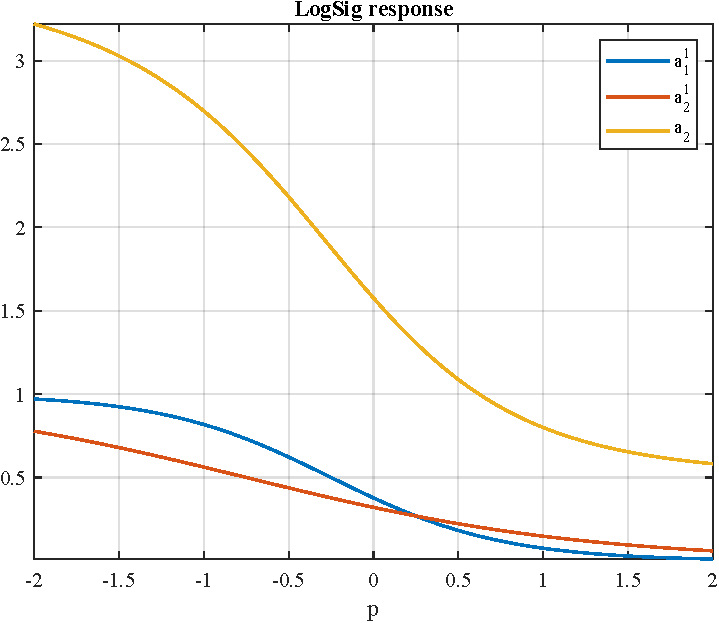
\includegraphics[width=\textwidth]{../Problem 5/logsig_activation.pdf}
	\end{subfigure}
	\hspace{1mm}
	\begin{subfigure}{0.47\textwidth}
		\centering
		\caption{}
		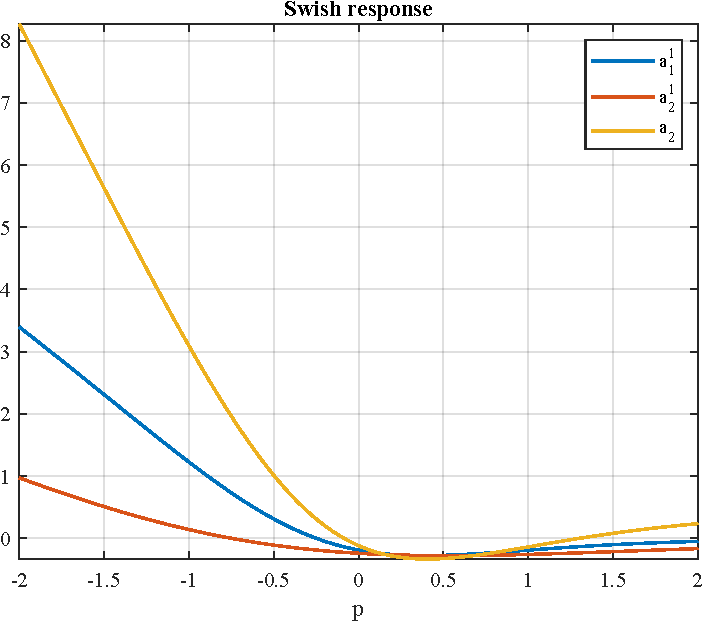
\includegraphics[width=\textwidth]{../Problem 5/swish_activation.pdf}
	\end{subfigure}
	\caption{Responses of different outputs of the neural network}
	\label{fig:prob_5_responses}
\end{figure}
	% !TeX spellcheck = en_US
\section{Problem 7}
\subsection{Question a}
Let a generic activation function be
\begin{equation}
S(x) = \left\{
\begin{array}{cc}
	x^k, & x>L\\[1mm]
	x^k \dfrac{\left(L+x\right)^m}{\left(L+x\right)^m + \left(L-x\right)^m}, & \left|x\right| \le L\\[1mm]
	0, & x < -L
\end{array}
\right.
\end{equation}
This function has some parameters $k,L,m$ called hyperparameters. By using them, this function can approximate others.

\subsubsection{Swish}
%Swish: $k=1, \ L=2e, \ m=e$\\
In order for our activation function to approximate Swish, we have to see the latter first.
Swish's function is 
\[
S(x) = \dfrac{x}{1+e^{-x}} = x\dfrac{e^x}{1+e^x}
\]
and is plotted in figure~\ref{fig:prob7_swish}. In order to determine the parameters, we have to take a look in the plotted function. When $x>0$, Swish seems to be almost $y=x$, thus $k=1$. If we look at $x<0$, we can se that Swish curves until it settles back to 0.
That point $x_1$ where $Swish (x_1) = 0$ is parameter $L$. After trying multiple values, we opted with $2e$ as this gives the smaller overall error in that region.
After filling $k,L$, only parameter $m$ is left to be found. In general, $x^e$ is a good approximation of $e^x$, but an approximation only. Just trying $m=e$ and plotting the created function gets us the plot in figure~\ref{fig:prob7_swish} which is really close to Swish.
Finally, the activation function can be written 
\[
S(x) = \left\{
\begin{array}{cc}
	x, & x>2e\\[1mm]
	x \dfrac{\left(2e+x\right)^e}{\left(2e+x\right)^e + \left(2e-x\right)^e}, & \left|x\right| \le 2e\\[1mm]
	0, & x < -2e
\end{array}
\right.
\]

\begin{figure}[H]
	\centering
	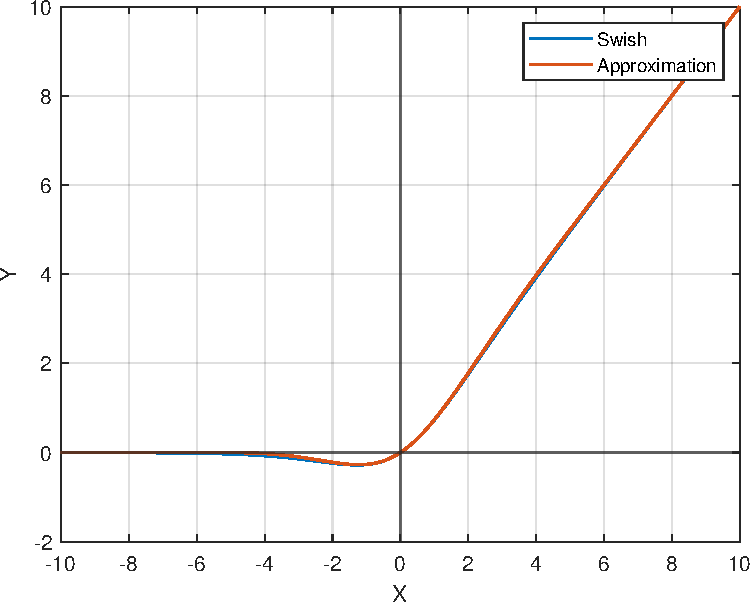
\includegraphics[width=.5\textwidth]{../Problem 7/prob7_swish.pdf}
	\caption{Swish activation function and its approximation.}
	\label{fig:prob7_swish}
\end{figure}

\subsubsection{Sigmoid}
Sigmoid's function is 
\[
S(x) = \dfrac{1}{1+e^{-x}} = \dfrac{e^x}{1+e^x}
\]
Just from this type, we understand that is $\frac{Swish(x)}{x}$. So, selecting parameters is easier this time as $m$ and $L$ will not change. Because of the previous equation, parameter $k$ must be decreased by $1$, thus $k=0$. Figure~\ref{fig:prob7_sigmoid} shows both the sigmoid and its approximation.

\begin{figure}[H]
	\centering
	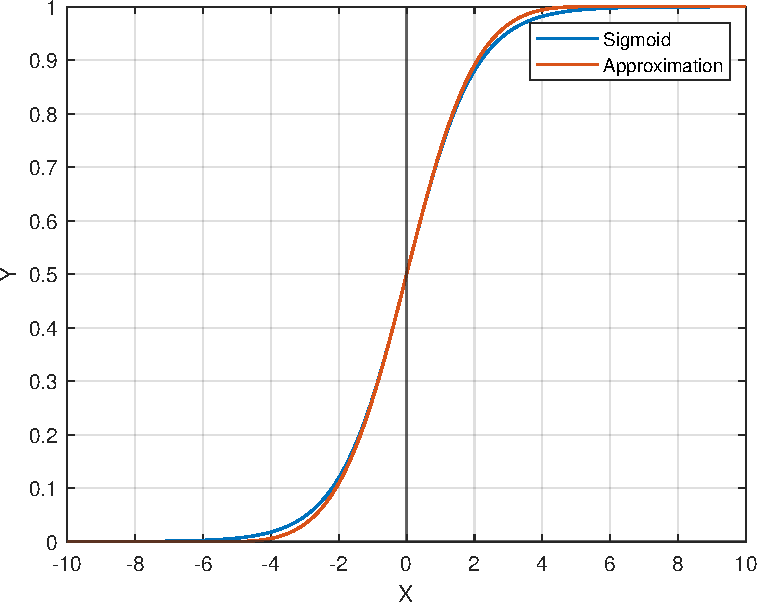
\includegraphics[width=.5\textwidth]{../Problem 7/prob7_sigmoid.pdf}
	\caption{Sigmoid activation function and its approximation.}
	\label{fig:prob7_sigmoid}
\end{figure}


\subsubsection{ReLU}
ReLU is defined as 
\[
ReLU(x) = \max(0,x) = \left\{
\begin{array}{cc}
	0, & x<0\\
	x, & x \ge 0
\end{array}
\right.
\]
From this, we can already determine parameter $k$ to be $k=1$, as we want $x^k = x \Rightarrow k=1$.
Setting $L=0$ ensures that the transition point between the linear and non-linear parts of the function occurs at $x=0$, which is consistent with the behavior of ReLU.
Also, setting $m=0$ means that the denominator term becomes $1$ for both the linear and non-linear parts of the function, simplifying the expression.
The plotted functions are presented in figure~\ref{fig:prob7_relu}\\
With parameters those mentioned above, $S(x)$ is the following
\[
S(x) = \left\{
\begin{array}{cc}
	x, & x\ge 0\\
	0, & x < 0
\end{array}
\right.
\]

\begin{figure}[H]
	\centering
	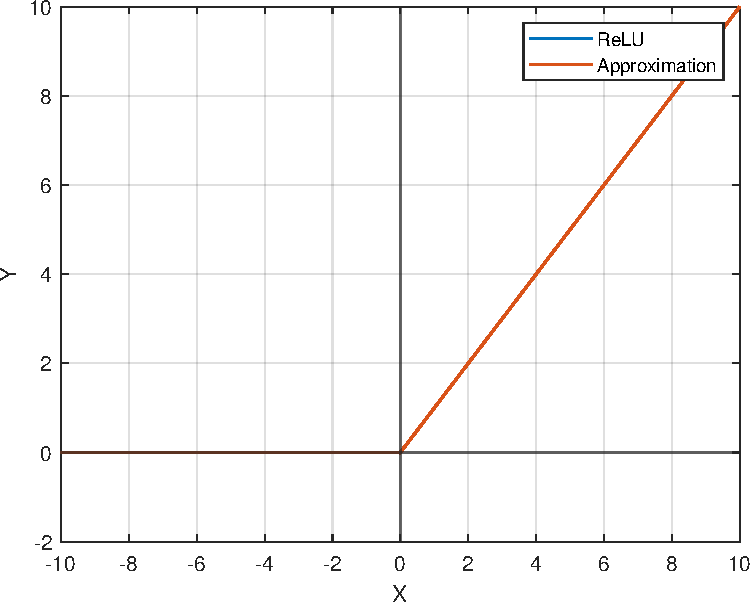
\includegraphics[width=0.5\textwidth]{../Problem 7/prob7_relu.pdf}
	\caption{ReLU activation function and its approximation.}
	\label{fig:prob7_relu}
\end{figure}

\subsubsection{ELU}
ELU's equation is 
\[
S(x) = \left\{
\begin{array}{cc}
	x, & x \ge 0\\
	\alpha \left(e^x - 1\right), & x<0\\
\end{array}
\right., \quad \text{with} \ \alpha=\left(0.1...0.3\right)
\]
From the equation above we understand that this activation function is almost the same as ReLU, with only difference being treatment of negative numbers. So, we can choose the same parameters from ReLU and still be a fairly good approximation to ELU, thus $k=1,\ L=0,\ m=0$.
Both ELU and it's approximation are presented in figure~\ref{fig:prob7_elu}.

\begin{figure}[H]
	\centering
	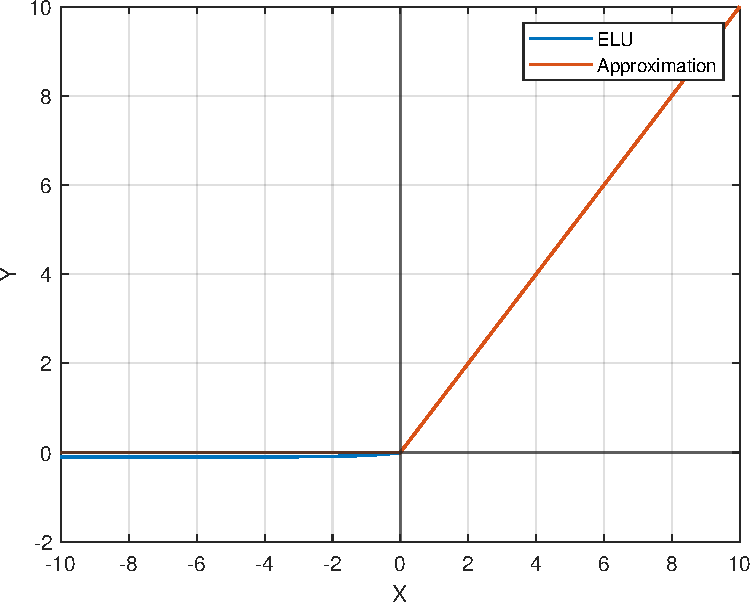
\includegraphics[width=0.5\textwidth]{../Problem 7/prob7_elu.pdf}
	\caption{ELU activation function and its approximation}
	\label{fig:prob7_elu}
\end{figure}


\subsection{Question b}
In order to make our calculations a bit easier, we set $g(x) = L+x$ and $i(x) = L-x$, with $\dfrac{dg(x)}{dx} = 1$, $\dfrac{di(x)}{dx} = -1$, $\dfrac{dg(x)}{dL} = 1$ and $\dfrac{di(x)}{dL} = 1$.

\subsubsection{Derivative with respect to x}
In $x \in \left[-L, L\right]$, the derivative is calculated as
\[
\begin{gathered}
\dfrac{dS(x)}{dx} = kx^{k-1} \dfrac{g^m(x)}{\left(g(x)+i(x)\right)^m} + \\[1mm]
+ x^k\dfrac{mg^{m-1}(x) \left( g^m(x) + i^m(x) \right) - g^m(x) \left( mg^{m-1}(x) - mi^{m-1}(x)\right)}{\left( g^m(x) + i^m(x) \right)^2} = \\[1mm]
= kx^{k-1} \dfrac{g^m(x)}{\left(g(x)+i(x)\right)^m} + x^k \dfrac{mg^m(x) i^m(x) \left( \frac{1}{g(x)} + \frac{1}{i(x)} \right)}{\left(g^m(x) + i(x)\right)^2}
\end{gathered}
\]

So, activation's function derivative is 
\begin{equation}
\frac{dS(x)}{dx} = \left\{
\begin{array}{cc}
	kx^{k-1} \ , & x>L\\[1mm]
	kx^{k-1} \dfrac{g^m(x)}{\left(g(x)+i(x)\right)^m} + x^k \dfrac{mg^m(x) i^m(x) \left( \frac{1}{g(x)} + \frac{1}{i(x)} \right)}{\left(g^m(x) + i(x)\right)^2}\ , & \left|x\right| \le L\\[1mm]
	0\ , & x<L
\end{array}
\right.
\end{equation}

\subsubsection{Derivative with respect to k}
We know from algebra that $\dfrac{d}{dx}\left(a^x\right) = a^x \ln a$. So
\[
\dfrac{dS}{dk} = x^k \ln (k) \dfrac{\left(L+x\right)^m}{\left(L+x\right)^m + \left(L-x\right)^m}, \quad \text{for } x \in \left[-L...L\right]
\]
Thus, the derivative is
\begin{equation}
\frac{dS(x)}{dk} = \left\{
\begin{array}{cc}
	x^k \ln(k) \ , & x>L\\[1mm]
 	x^k \ln (k) \dfrac{g^m(x)}{g^m(x) + i^m(x)}\ , & \left|x\right| \le L\\[1mm]
	0\ , & x<L
\end{array}
\right.
\end{equation}

\subsubsection{Derivative with respect to L}
This derivative is similar to that in respect to $x$, so calculating it gives us
\[
\dfrac{dS}{dL} = x^k \dfrac{mg^{m-1}(x) \left( g^m(x) + i^m(x) \right) - g^m(x) \left( mg^{m-1}(x) + mi^{m-1}(x)\right)}{\left( g^m(x) + i^m(x) \right)^2} = 0 
\]
So, 
\begin{equation}
	\dfrac{dS(x)}{dL} = 0, \ \text{for all different L}
\end{equation}

\subsubsection{Derivative with respect to m}
\[
\begin{gathered}
\dfrac{dS}{dm} = x^k\dfrac{g^{2m}(x) \ln(g(x)) +g^m(x) i^m(x) \ln (g(x)) - \left( g^{2m}(x) \ln(g(x)) + g^m(x) i^m(x) \ln(i(x)) \right)}{\left( g^m(x) + i^m(x)\right)^2} = \\[1mm]
= \dfrac{g^m(x) i^m(x) \ln(g(x)) - g^m(x) i^m(x) \ln(i(x))}{\left(  g^m(x) + i^m(x)\right)^2} 
= \dfrac{g^m(x) i^m(x) \ln\left(\frac{g(x)}{i(x)}\right)}{\left(  g^m(x) + i^m(x)\right)^2}
\end{gathered}
\]

Thus, the derivative of $S(x)$ with respect to m is 
\begin{equation}
\dfrac{dS}{dm} = \left\{
\begin{array}{cc}
	0 \ , & x>L\\[1mm]
	\dfrac{g^m(x) i^m(x) \ln\left(\frac{g(x)}{i(x)}\right)}{\left(  g^m(x) + i^m(x)\right)^2}\ , & \left|x\right| \le L\\[1mm]
	0\ , & x<L
\end{array}
\right.
\end{equation}

	% !TeX spellcheck = en_US

\section{Problem 8}
ADALINE is a single-layer artificial neural network that can learn and adapt to non-linear relationships between inputs and outputs. \\
It consists of a single neuron with a linear activation function. Each input of the neuron has a corresponding weight,which is adapted during training to minimize the error between the network's output and the desired output. To adjust the weights the algorithm uses the learning rule α.
\vspace{0.3cm}

Suppose that we have the following three reference patterns and their targets:
\vspace{5mm}

\[
\begin{array}{ccc}
%	\centering
	\left\{ 
	p_1 = \left[
	\begin{array}{c}
		2 \\
		4
	\end{array}
	\right], t_1 = \left[26\right]
	\right\} & 
	\left\{ 
	p_2 = \left[
	\begin{array}{c}
		4 \\
		2
	\end{array}
	\right], t_2 = \left[26\right]
	\right\}
	&\left\{ 
	p_3 = \left[
	\begin{array}{c}
		-2 \\
		-2
	\end{array}
	\right], t_3 = \left[-26\right]
	\right\}
	
\end{array}
\]

\vspace{5mm}

The probability of vector p1 is $P_{1}= 0.20$, the probability of vector p2 is $P_{2}= 0.70$, and the probability of vector p3 is $P_{3}= 0.10$.


\subsection{Question a}
The number of inputs to an ADALINE network for each neural network is determined by the dimensionality of our data,not by the number of patterns we have. In our case, each pattern is a 2-dimensional vector. Therefore, our ADALINE network has two inputs, one for each dimension.\\
In an ADALINE network, the number of weights is equal to the number of inputs. In our case, we have two inputs. Thus, our neural network has two weights, one for each dimension of the input.\\
From theory, the output of an ADALINE network is a = purelin($W_{p}$+b).\\

So, the network diagram for the given ADALINE network with no bias that will be trained with  these patterns is shown in figure \ref{fig:prob8_adaline_draw}.

\begin{figure}[htpb]
	\centering
	\includesvg[width=0.7\textwidth]{../Problem 8/problem8.svg}
	\caption{ADALINE neural network architecture}
	\label{fig:prob8_adaline_draw}
\end{figure}

\subsection{Question b}
In order to sketch the contour plot of the mean square error performance index, we first must calculate the various terms of the quadratic function.\\
Recall that, $ F(x) = c-2 \cdot x^T \cdot h + x^T \cdot R \cdot x $ where,
\begin{itemize}
	\item c: A scalar constant term. It shifts the function up or down along the y-axis.
	\item R: Correlation matrix of the input data. It determines the curvature of the function
	\item h: The cross-correlation between the input data and its associated target.  It determines the slope of the function.
	\item x: The vector of variables (or weights).
\end{itemize}
These parameters define the shape of the quadratic function. So,we must calculate c,h,R in relation to 
 \[x = \left[
\begin{array}{cc}  
  	W_{11} & W_{12} \\  
\end{array}
\right]
\]

The calculations:
\[ 
\begin{gathered}
	c = E[t^2] = t_1^2 \cdot p_1 + t_2^2 \cdot p_2 + t_3^2 \cdot p_3 = 26^2 \cdot 0.2 + 26^2 \cdot 0.7 + (-26)^2 \cdot 0.1\\
	\rightarrow c = 676
\end{gathered}
\]
\[
\begin{gathered}
h = E[t \cdot p] = P_1 \cdot t_1 \cdot p_1 + P_2 \cdot t_2 \cdot p_2 + P_3 \cdot t_3 \cdot p_3 = \\ 0.2 \cdot 26 \cdot \left[
\begin{array}{cc}  
	2 \\  
	4 \\
\end{array}
\right] + 0.7 \cdot 26 \cdot \left[ \begin{array}{cc}  
	4 \\  
	2 \\
\end{array}
\right] + 0.1 \cdot (-26) \cdot \left[ \begin{array}{cc}  
	-2 \\  
	-2 \\
\end{array}
\right] \\
\rightarrow h = \left[
	\begin{array}{c}  
		88.4 \\  
		62.4 \\
	\end{array}
	\right]
\end{gathered}
\]
\\
\[
\begin{gathered}
	R = E[p \cdot p^T] = P_1 \cdot p_1 \cdot p_1^T + P_2 \cdot p_2 \cdot p_2^T + P_3 \cdot p_3 \cdot p_3^T \\ = 0.2 \cdot \left[
	\begin{array}{c}  
		2 \\  
		4 \\
	\end{array}
	\right] \cdot \left[
	\begin{array}{c}  
		2 \\  
		4 \\
	\end{array}
	\right]^T +  0.7 \cdot \left[
	\begin{array}{c}  
		4 \\  
		2 \\
	\end{array}
	\right] \cdot \left[
	\begin{array}{c}  
		4 \\  
		2 \\
	\end{array}
	\right]^T +  0.1 \cdot \left[
	\begin{array}{c}  
		-2 \\  
		-2 \\
	\end{array}
	\right] \cdot \left[
	\begin{array}{c}  
		-2 \\  
		-2 \\
	\end{array}
	\right]^T \\
	\rightarrow R = \left[
	\begin{array}{cc}
		12.4 & 7.6 \\
		7.6 & 6.4
	\end{array}
	\right]	
\end{gathered}
\]
\vspace{2mm}
In conclusion the Mean Square Error (MSE) performance index is:
\[
F(x) = 676 - 2 \cdot \left[\begin{array}{cc}
	W_{11} & W_{12}
\end{array}
\right] \cdot \left[\begin{array}{c}
	88.4 \\
	62.4
\end{array}
\right] + \left[\begin{array}{cc}
	W_{11} & W_{12}
\end{array}
\right] \cdot \left[
\begin{array}{cc}
	12.4 & 7.6 \\
	7.6 & 6.4
\end{array}
\right]	\cdot \left[\begin{array}{c}
	W_{11} \\
	W_{12}
\end{array}
\right] \rightarrow
\]

\[
F(x) = 676 -176.8 \cdot W_{11} - 124.8 \cdot W_{12} + 12.4 \cdot W_{11}^2 + 15.2 \cdot W_{11}\cdot W_{12} + 6.4 \cdot W_{12}^2
\]
\\
By inserting this function into Matlab we get the 2D and 3D contour plots of the MSE index
as shown in figures \ref{fig:prob_8_2d} and \ref{fig:prob_8_3d}
\begin{figure}[H]
	\centering
	\begin{subfigure}{0.47\textwidth}
		\centering
		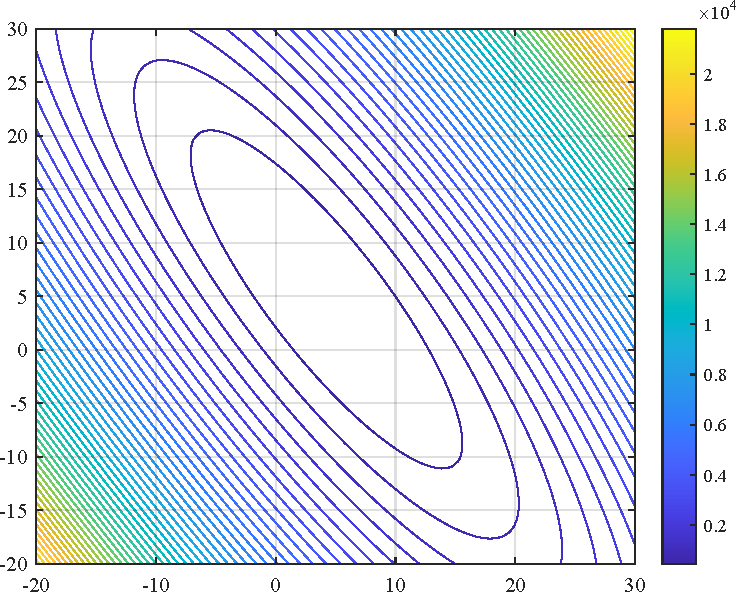
\includegraphics[width=\textwidth]{../Problem 8/contour_2d.pdf}
		\caption{2D plot of MSE index}
		\label{fig:prob_8_2d}
	\end{subfigure}
	\hspace{2mm}
	\begin{subfigure}{0.47\textwidth}
		\centering
		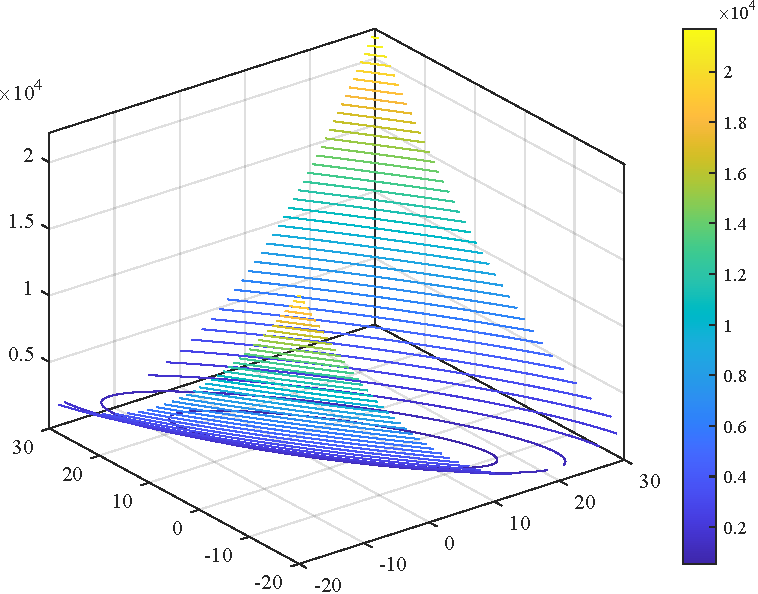
\includegraphics[width=\textwidth]{../Problem 8/contour_3d.pdf}
		\caption{3D plot of MSE index}
		\label{fig:prob_8_3d}
	\end{subfigure}	
\end{figure}

\subsection{Question c}
A decision boundary is a hypersurface that separates different classes in a classification problem.\\
For a binary classification problem,as in our case, all points on one side of the decision boundary are predicted to belong to one class, while points on the other side are predicted to belong to the other class.\\
The optimal decision boundary is the one that minimizes a certain transfer function. Here it is a line that can be described by the equation 
\[
\begin{gathered}
	f(x) = W^T \cdot x^*, 
\end{gathered}
\]
where $
W=\left[\begin{array}{cc}
	W_{11} & W_{12}
\end{array}
\right]
$ and $x^*$ the minimum square error \\
$x^*$ is the strong minimum, a stationary point that is indeed the center of the cycle of Figure \ref{fig:prob_8_2d}.\\

So, in order to find the optimal decision boundary we follow the mentioned steps:
\begin{itemize}
	\item $f(x) = W^T \cdot x^*$
	\item Set f(x) = 0
	\item Calculate $x^* = R^-1 \cdot h$
	\item Replace the value in f(x)
\end{itemize}

By calculating $x^* = R^-1 \cdot h$ we get that $x^* = \left[\begin{array}{c}
															4.2370 \\
															4.7185 \\
														\end{array}
														\right] $

\vspace{5mm}
and the optimal decision boundary is $f(W_{11},W_{12}) = 4.2370 \cdot W_{11} + 4.7185 \cdot W_{12} $ \\

With the help of Matlab we get the following figure \ref{fig:patterns}

\begin{figure}[H]
	\centering
	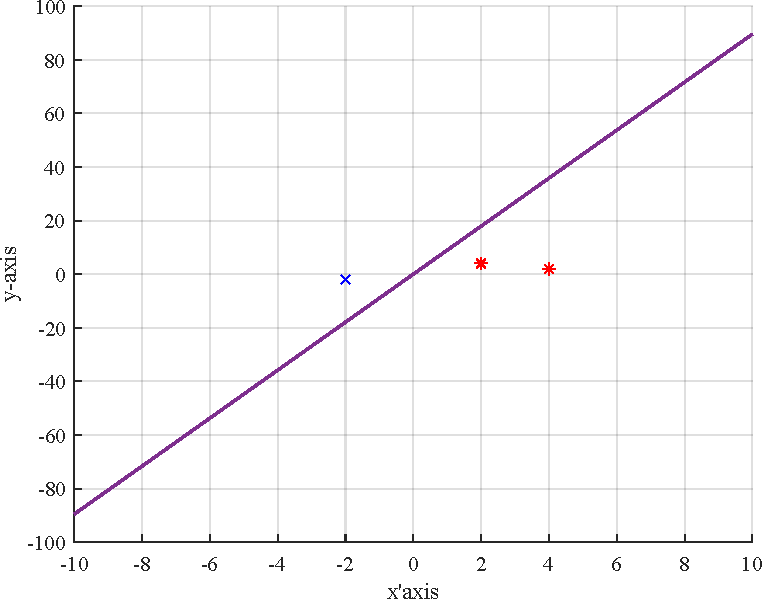
\includegraphics[width = 0.6\textwidth]{../Problem 8/patterns.pdf}
	\caption{Optimal Decision Boundary line and the patterns}
	\label{fig:patterns}
\end{figure}





	


	% !TeX spellcheck = en_US


\section{Problem 9}
Again, suppose that we have the following two reference patterns and their targets:
\vspace{5mm}

\[
\begin{array}{ccc}
	%	\centering
	\left\{ 
	p_1 = \left[
	\begin{array}{c}
		1 \\
		2
	\end{array}
	\right], t_1 = \left[-1\right]
	\right\} & 
	\left\{ 
	p_2 = \left[
	\begin{array}{c}
		-2 \\
		1
	\end{array}
	\right], t_2 = \left[1\right]
	\right\}
\end{array}
\]
\vspace{5mm}

The probabilities of vectors $p_1$ and $p_2$ are equiprobable, so that means $P_1 = P_2 = 0.5$.

\subsection{Question a}
In order to sketch the contour plot of the Mean Square Error performance, we ought to calculate the arguments of the quadratic function F(x). As we did on Problem8-Question \ref{Questionb}, with the help of Matlab we calculate the c,R,h and we get the following results\\

\begin{itemize}
	\item $R = \left[
	\begin{array}{cc}
		2.5 & 0 \\
		0 & 2.5 \\
	\end{array}
	\right]
	$
	\item $h = \left[
	\begin{array}{c}
		-1.5 \\
		-0.5
	\end{array}
	\right]
	$
	\item c = 1
\end{itemize}
and the MSE function is:
$F(x) = 1 - 3 \cdot w_{11} -w_{12} + 2.5 \cdot w_{11}^2 + 2.5 \cdot w_{12}^2$ \\

From the form of the equation we can understand that it is a circle with a center of $x^* = R^-1 \cdot h.$\\
By the Matlab code that i provided to calculate the F(x), we get the 2D and 3D contour plots of the MSE index as shown in figures \ref{fig:prob_9_2d} and \ref{fig:prob_9_3d}\\
\begin{figure}[H]
	\centering
	\begin{subfigure}{0.47\textwidth}
		\centering
		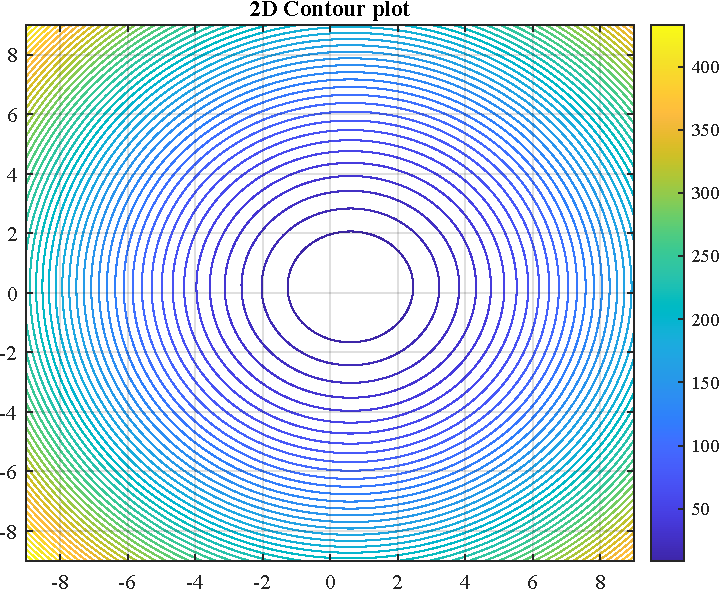
\includegraphics[width=\textwidth]{../Problem 9/contour_2d.pdf}
		\caption{2D plot of MSE index}
		\label{fig:prob_9_2d}
	\end{subfigure}
	\hspace{2mm}
	\begin{subfigure}{0.47\textwidth}
		\centering
		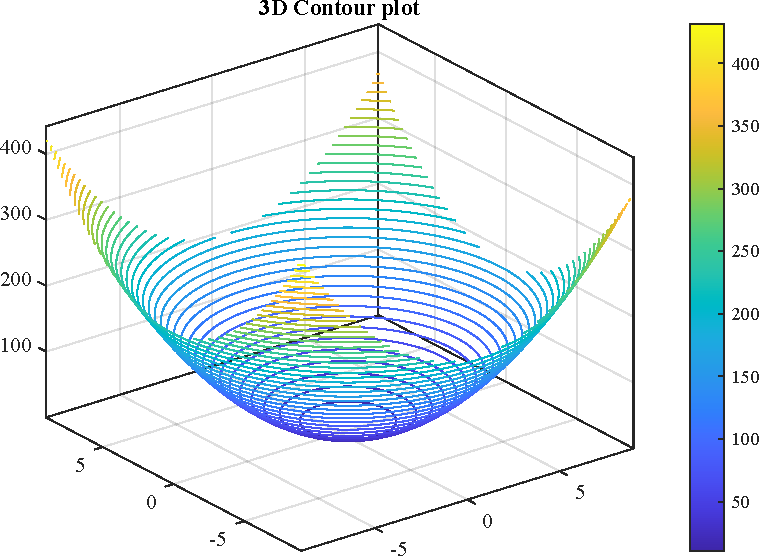
\includegraphics[width=\textwidth]{../Problem 9/contour_3d.pdf}
		\caption{3D plot of MSE index}
		\label{fig:prob_9_3d}
	\end{subfigure}	
\end{figure}

\subsection{Question b}
Working with the same method as i did in Problem8-Question \ref{Questionc} but this time with the help of Matlab code, we got the following sketch about the optimal decision boundary.

\begin{figure}[H]
	\centering
	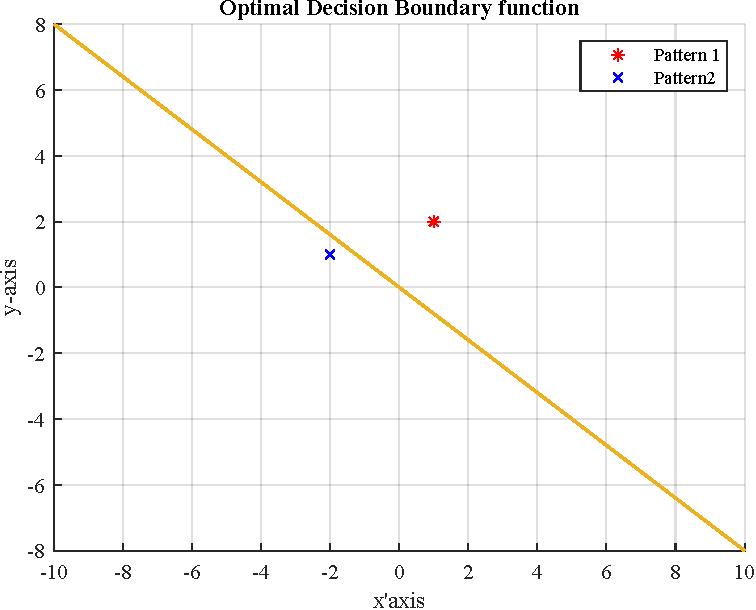
\includegraphics[width=0.5\textwidth]{../Problem 9/patterns.pdf}
	\caption{Optimal decision Boundary plot}
	\label{fig:OpDecBo}
\end{figure}

We can verify that indeed the optimal decision boundary separates and correctly classifies the patterns.

\subsection{Question c}
If we want to sketch the trajectory of the LMS algorithm on our contour plot, we follow the methodology of Problem8- Question\ref{Questione}, but for the number of iterations N = 100.\\
Here our learning rate is lr = 0.025 and the initial weight is $w(0) = \left[
\begin{array}{c}
	3 \\
	1
\end{array}
\right]
$

Using Matlab, we exported this trajectory of the LMS algorithm to our 2D contour plot of the mean square error performance index.
\begin{figure}[H]
	\centering
	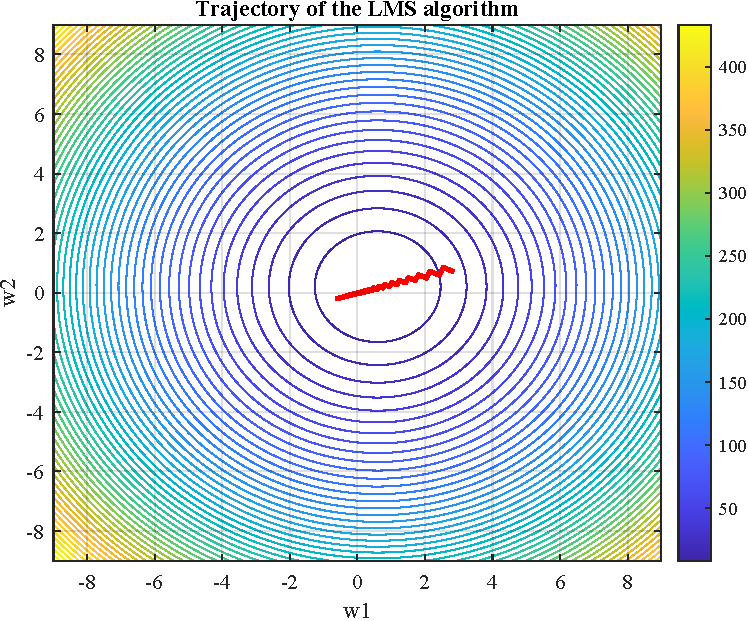
\includegraphics[width=0.45\textwidth]{../Problem 9/contour_2d_traj.pdf}
	\caption{Trajectory of the LMS algorithm}
	\label{fig:trajectory}
\end{figure}



	% !TeX spellcheck = en_US
\section{Problem 10}

\subsection{Question A}

The patterns that we want to separate are plotted in figure~\ref{fig:prob_10_patterns}.

\begin{figure}[htpb]
	\centering
	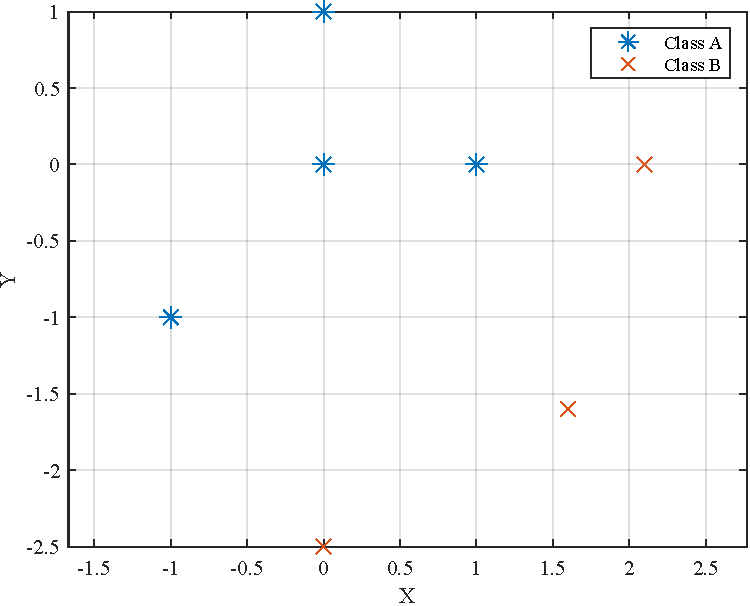
\includegraphics[width=0.5\textwidth]{../Problem 10/patterns.pdf}
	\caption{Plot of patterns}
	\label{fig:prob_10_patterns}
\end{figure}

We can clearly see that there can be a straight line that can separate the two classes, thus an ADALINE neural network can work in classification for this system.

\subsection{Question B}

The designed ADALINE neural network will be of the following architecture
\begin{itemize}
	\item Input Layer: Since the patterns are two-dimensional (each pattern has two values), the input layer will have two nodes.
	\item Output Layer: The output layer will have one node. This is because the task is a binary classification (Class A or Class B). The output node will use a linear activation function, as is standard in ADALINE networks.
	\item Weights and Bias: There will be two weights (one for each input node) and one bias. The weights and bias are parameters that the network will learn during the training process.
	\item Learning Rule: The network will use the LMS learning rule (\textit{Least Mean Square}) to update the weights and bias. This rule minimizes the mean square error between the network's output and the target output.
\end{itemize}

This architecture described beforehand is shown in figure~\ref{fig:prob10_adaline_architecture}.
\begin{figure}[htpb]
	\centering
	\includesvg[width=0.5\textwidth]{../Problem 10/prob10_adaline.svg}
	\caption{ADALINE neural network architecture}
	\label{fig:prob10_adaline_architecture}
\end{figure}
	% !TeX spellcheck = en_US
\section{Problem 11}

Fuzzy logic is a type of logic that deals with vague, imprecise, or uncertain information. It is based on the concept of fuzzy sets, which are sets that can have any degree of membership between 0 and 1.  The value zero is used to represent complete non-membership, the value one is used to represent complete membership, and values in between are used to represent intermediate degrees of membership.This means that an element can be a member of a fuzzy set to some degree, rather than all or nothing.

The uniqueness of fuzzy logic is that fuzzy logic can handle imprecise and uncertain information,which makes it a valuable tool for dealing with real-life problems that are inherently vague or fuzzy. 

On this exercise, we are dealing with the linguistic variable \textit{Truth} with a possible membership set: 

\begin{center}
	\textit{T = {Absolutely false, Very false, False, Fairly true, True, Very true, Absolutely true}}
\end{center}

Based on that set we may define the membership function of truth as:
\begin{center}
	\textit{True(u) = u \hspace{3mm}  False(u) = 1-u}
\end{center}
for each $u \in [0, 1]$.

	






	% !TeX spellcheck = en_US
\section{Problem 12}

In order to evaluate the expression "\verb|not(A(x) OR B(x))|", we first have to take a look in how fuzzy logic is different with binary logic at the operation level.
In binary logic we have three basic operations: \verb*|AND(x,y)|, \verb*|OR(x,y)| and \verb*|NOT(x)|. But, in fuzzy logic, where a function can have a value in range of $\left[0...1\right]$, things are a bit different.
Operation \verb*|AND(x,y)| of binary is equivalent with \verb|MIN(x,y)| from the fuzzy logic, \verb*|OR(x,y)| with \verb*|MAX(x,y)| and \verb*|NOT(x)| with \verb|1-x|.

\begin{wrapfigure}{R}{0.5\textwidth}
	\centering
	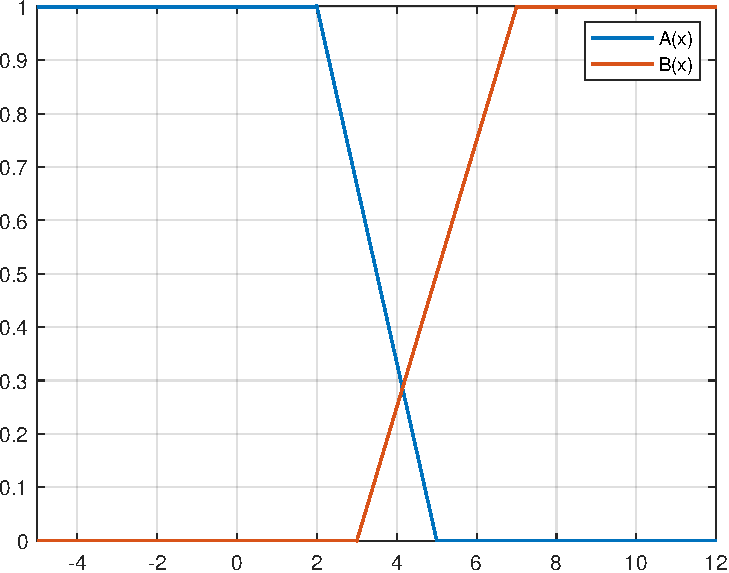
\includegraphics[width=0.4\textwidth]{../Problem 12/a_b_functions.pdf}
	\caption{Plot of A(x), B(x)}
	\label{fig:prob_12_a_b}
\end{wrapfigure}

We have to find the proper $x$ for which the previous expression has the greater value. Firstly, we will calculate the expression and then find the proper $x$.
To achieve this, we will have to break down our calculations in areas. 

Starting with $x \le 2$, $"A(x) \text{ AND } B(x)"$ is equal to $"\max\left(A(x), B(x)\right)" = 1$. So, using De Morgan's law, we have $\textit{max}\left(A(x), B(x)\right) = \textit{not}\left(A(x) \textit{ or } B(x)\right) = 0$.
The exact same result is obtained at $x \ge 7$.

Things are a bit different in $2 \le x \le 7$. Function $A(x)$ starts to fall while $B(x)$ starts to rise. The point where they cross is valuable for defining the expression needed and can be found by solving the equation 
\[
A(x) = B(x) \Leftrightarrow 1 - \frac{x-2}{3} = \frac{x-3}{4} \Rightarrow x = \frac{29}{7}
\]

So, for $2 \le x \le \frac{29}{7}$, $\textit{max}\left(A(x), B(x)\right) = 1 - \dfrac{x-2}{3} = A(x)$, because in this region $A(x)$ is above $B(x)$. Thus, $\textit{not}\left(A(x) \textit{ or } B(x)\right) = \dfrac{x-2}{3}$.

Using the same logic, we find out that for $\frac{29}{7} \le x \le 7$, $\textit{not}\left(A(x) \textit{ or } B(x)\right) = 1 - \dfrac{x-3}{4}$. 

Therefore, the expression $f(x) = \textit{not}\left(A(x) \textit{ or } B(x)\right)$ is summarized in the following:
\begin{equation}
	f(x) = \left\{
	\begin{array}{cc}
		0 & x \le 2, \\[3pt]
		\dfrac{x-2}{3} & 2 \le x \le \frac{29}{7}, \\[7pt]
		1 - \dfrac{x-3}{4} & \frac{29}{7} \le x \le 7, \\[3pt]
		0 & x \ge 7\\
	\end{array}
	\right.
\end{equation}
	
\end{document}